\documentclass{beamer}

\usepackage[utf8]{inputenc}
\usepackage{lmodern} 
\usepackage[utf8]{inputenc}
\usepackage{lmodern} 
\usepackage{listings}
\usepackage{xcolor} 
\usepackage{graphicx}
\definecolor{myblue}{RGB}{48, 63, 159}
\setbeamercolor{palette primary}{bg=myblue, fg=white}
\setbeamercolor{structure}{fg=myblue}
\setbeamercolor{frametitle}{bg=myblue, fg=white}
\setbeamercolor{title}{bg=myblue, fg=white}
\setbeamercolor{footlinecolor}{bg=myblue, fg=white}


\defbeamertemplate*{title page}{mytemplate}{
	\vfill
	\begin{center}
		
		\begin{beamercolorbox}[wd=0.8\paperwidth, center, rounded=true, shadow=true]{title}
			\usebeamerfont{title}\inserttitle\par
		\end{beamercolorbox}
		\vspace{2cm} 
		
		\usebeamerfont{author}\insertauthor
		\vspace{1cm} 
		\usebeamerfont{date}\insertdate
	\end{center}
	\vfill
}


\defbeamertemplate*{frametitle}{mytemplate}{
	\begin{beamercolorbox}[wd=\paperwidth, ht=2.5ex, dp=1.5ex, left]{frametitle}
		\hspace{1em}\usebeamerfont{frametitle}\insertframetitle
	\end{beamercolorbox}
}


\setbeamertemplate{footline}{
	\begin{beamercolorbox}[wd=\paperwidth, ht=2.25ex, dp=1ex]{footlinecolor}
		\hspace{1em}\usebeamerfont{author in footline}\insertshortauthor
		\hfill
		\usebeamerfont{title in footline}\insertshorttitle
		\hfill
		\usebeamerfont{date in footline}\insertdate \hspace{1em} \insertframenumber/\inserttotalframenumber \hspace{0.5em}
	\end{beamercolorbox}
}


\setbeamerfont{author in footline}{size=\tiny}
\setbeamerfont{title in footline}{size=\tiny}
\setbeamerfont{date in footline}{size=\tiny}

\newcommand{\myvec}[1]{\ensuremath{\begin{pmatrix}#1\end{pmatrix}}}
\providecommand{\brak}[1]{\ensuremath{\left(#1\right)}}


\title{4.13.57}
\author{Shriyansh Chawda-EE25BTECH11052}
\date{August 23, 2025}



\begin{document}
	

		\setbeamertemplate{footline}{} 
		\frame{\titlepage}
	
	
	

	\begin{frame}{Question} 
Find the equation of the line passing through the point $(2,3)$ and making intercept of length 2 units between the lines $y + 2x = 3$ and $y + 2x = 5$. 
\hfill(1991)
\begin{figure}[H]
	\centering
	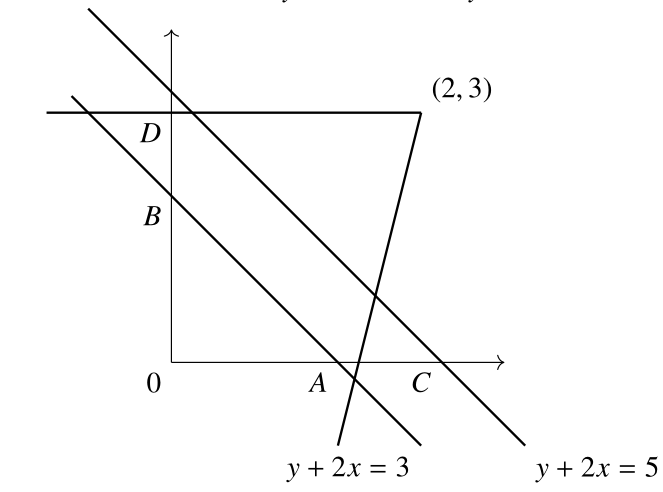
\includegraphics[width=0.5\linewidth]{figs/question}
	\end{figure}
\end{frame}
	
\begin{frame}{Solution}
The point is given by:
\[ \mathbf{P} = \myvec{2 \\ 3} \]
The two lines are expressed in the vector form $\mathbf{n} \cdot \mathbf{x} = d$.
\begin{align}
	\myvec{2 & 1} \myvec{x \\ y} = 3 \\
	\myvec{2 & 1} \myvec{x \\ y} = 5
\end{align}
The common normal vector is $\mathbf{n}$ and the distance constants $d_1$ and $d_2$:
\begin{align}
	\mathbf{n} = \myvec{2 \\ 1}, \quad d_1 = 3, \quad d_2 = 5 \end{align}
	The line passes through $\mathbf{P}$ with an unknown direction vector $\mathbf{v}$ is:
\end{frame}

\begin{frame}{Solution}
\begin{align} \mathbf{x} = \mathbf{P} + t\mathbf{v} = \myvec{2 \\ 3} + t \myvec{v_x \\ v_y} \end{align}
The unknown line intersect $L_1$ at point $\mathbf{B}$ (parameter $t_B$) and $L_2$ at point $\mathbf{D}$ (parameter $t_D$).
\begin{align}
	\mathbf{n} \cdot (\mathbf{P} + t_B \mathbf{v}) = d_1 &\implies t_B = \frac{d_1 - \mathbf{n} \cdot \mathbf{P}}{\mathbf{n} \cdot \mathbf{v}} \\
	\mathbf{n} \cdot (\mathbf{P} + t_D \mathbf{v}) = d_2 &\implies t_D = \frac{d_2 - \mathbf{n} \cdot \mathbf{P}}{\mathbf{n} \cdot \mathbf{v}}
\end{align}
Now ,Using the length of intercept.\\
\begin{align}
	\|\mathbf{D} - \mathbf{B}\| = \|(\mathbf{P} + t_D \mathbf{v}) - (\mathbf{P} + t_B \mathbf{v})\| = |t_D - t_B| \cdot \|\mathbf{v}\| = 2
\end{align} 	
\end{frame}

\begin{frame}{Solution}
Using (0.3) and (0.4)\\
\begin{align}
	t_D - t_B = \frac{d_2 - \mathbf{n} \cdot \mathbf{P}}{\mathbf{n} \cdot \mathbf{v}} - \frac{d_1 - \mathbf{n} \cdot \mathbf{P}}{\mathbf{n} \cdot \mathbf{v}} = \frac{d_2 - d_1}{\mathbf{n} \cdot \mathbf{v}}
\end{align}
Substituting this into the distance equation:
\begin{align}
	\left| \frac{d_2 - d_1}{\mathbf{n} \cdot \mathbf{v}} \right| \cdot \|\mathbf{v}\| = 2 \\
	\frac{2}{|\mathbf{n} \cdot \mathbf{v}|} \cdot \|\mathbf{v}\| = 2 \implies \|\mathbf{v}\| = |\mathbf{n} \cdot \mathbf{v}| 
\end{align}
We express the condition $\|\mathbf{v}\| = |\mathbf{n} \cdot \mathbf{v}|$ as a matrix quadratic form. Squaring both sides gives:
\end{frame}

\begin{frame}{Solution}
\begin{align} 
	&\|\mathbf{v}\|^2 = (\mathbf{n} \cdot \mathbf{v})^2 \\
	&\mathbf{v}^\top\mathbf{I}\mathbf{v} = \mathbf{v}^\top(\mathbf{n}\mathbf{n}^\top)\mathbf{v} \\
	&\mathbf{v}^\top\mathbf{I}\mathbf{v} - \mathbf{v}^\top(\mathbf{n}\mathbf{n}^\top)\mathbf{v} = 0\\
	&\mathbf{v}^\top (\mathbf{n}\mathbf{n}^\top - \mathbf{I}) \mathbf{v} = 0, 
\end{align}
Let,
\begin{align}
	\mathbf{Q} = \mathbf{n}\mathbf{n}^\top - \mathbf{I} = \myvec{2 \\ 1} \myvec{2 & 1} - \myvec{1 & 0 \\ 0 & 1} = \myvec{3 & 2 \\ 2 & 0} 
\end{align}
We now solve the quadratic form equation for $\mathbf{v} = \myvec{v_x \\ v_y}$:
\begin{align} \mathbf{v}^\top \mathbf{Q} \mathbf{v} = \myvec{v_x & v_y} \myvec{3 & 2 \\ 2 & 0} \myvec{v_x \\ v_y} = 0 \end{align}
\end{frame}

\begin{frame}{Solution}
\begin{align} 
	3v_x^2 + 4v_xv_y = 0 \implies v_x(3v_x + 4v_y) = 0 
\end{align}
This yields two possible solutions for the components of the direction vector.\\
(a) $v_x = 0$ : The direction vector is vertical.Hence $\mathbf{v_1}$ and vertical line passing through the point $(2, 3)$ is :
\begin{align} 
	&\mathbf{v_1} = \myvec{0 \\ 1}\\
	&\mathbf{x} = 2 
\end{align}
(b) $3v_x + 4v_y = 0$ : This implies \begin{align}
	v_y = -\frac{3}{4}v_x\\
	\mathbf{v_2} = \myvec{4 \\ -3}
\end{align}
\end{frame}

\begin{frame}{Solution}
So, corresponding to a slope of $m = -3/4$. Using the point-slope form :
\begin{align}
	&y - 3 = -\frac{3}{4}(x - 2) \\
	&4(y - 3) = -3(x - 2) \\
	&4y - 12 = -3x + 6 \\
	&3x + 4y = 18
\end{align}
The two lines that satisfy the given conditions are :
\[	x = 2 \quad and\quad
3x + 4y = 18 \]
\end{frame}

\begin{frame}{Plot}
\begin{figure}
	\centering
	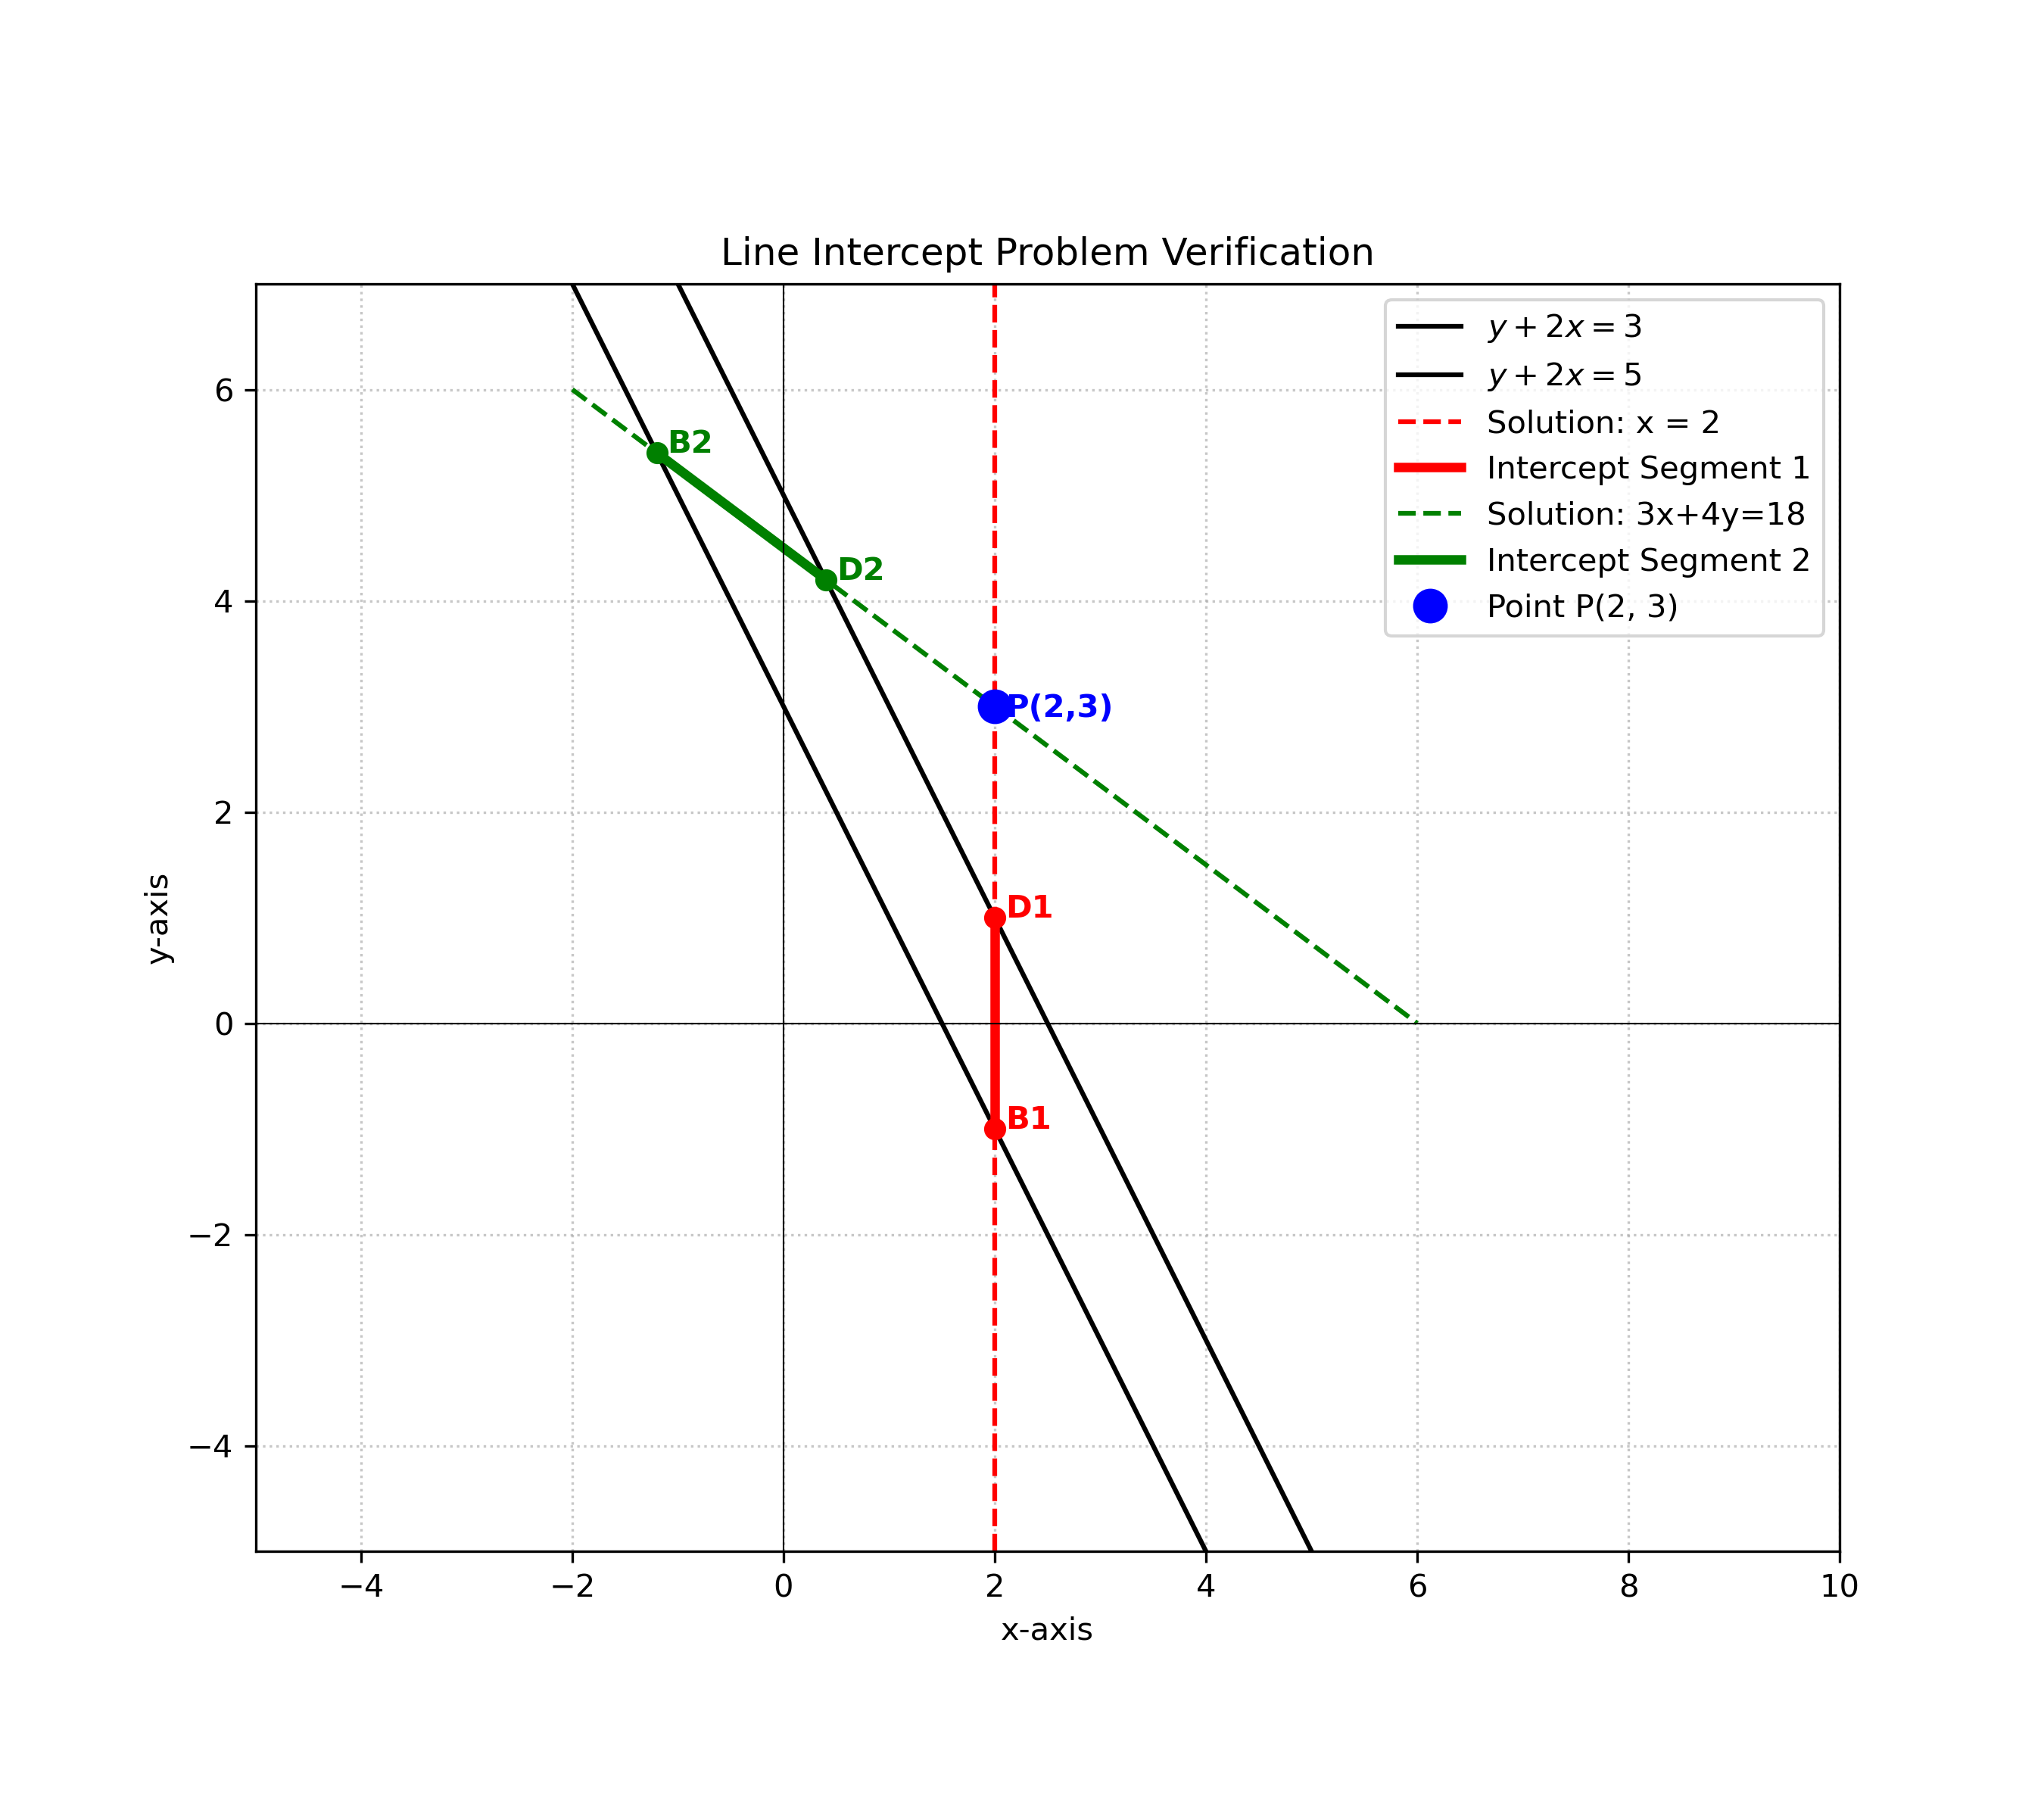
\includegraphics[width=1\linewidth]{figs/line_intercept_plot}
	\caption{}
	\label{fig:lineinterceptplot}
\end{figure}

\end{frame}

\end{document}